%!TEX root = principal.tex
\section{Dispositivos Eletromecânicos}

Há vários dispositivos eletromecânicos de interesse para a automação industrial, dos quais destacamos motores elétricos, solenóides, chaves e relês.

Destes, motores e solenóides são atuadores e chaves são sensores. Relês podem ser usados tanto como atuadores como como sensores, embora sejam mais usados em atuadores.

Chaves já foram vistas junto com instrumentação, enquanto motores são assuntos de outras disciplinas e fogem do escopo desta disciplian.

Solenóides são basicamente eletroimãs com um eixo ferromagnético preso a uma mola. O eixo pode ter duas posições: uma mantida pela mola, que é a posição que ele assume quando o eletroimã não é acionado, e outra forçando a mola, quando o eletroimã é acionado. Ou seja: são dispositivos de acionamento binários.

Solenóides tipicamente fornecem uma movimentação de no máximo poucos centímetros a cargas de miligramas a dezenas de kilogramas. São muito usados para acionamento de válvulas - válvulas solenóides.

Relês eletromecânicos são, por construção, solenóides no qual o eixo faz abrir ou fechar contatos elétricos. Eles são chaves elétricas acionadas eletricamente. Hoje em dia existem relês baseados em eletrônica, chamados de relês de estado sólido, que tem a mesma função mas por princípios de funcionamento bem diferentes. Eletricamente pode-se visualizar um relê apenas como um indutor (a bobina do eletroimã) e um contato, e muitas vezes é desta forma que ele é representado em um diagrama esquemático (vide exemplo na Figura \ref{fig:diagRele}).

O estado de repouso dos cantatos define o tipo básico do relê: normalmente aberto ou normalmente fechado. É comum relês que tenham 2 ou mais contatos acionadas por uma mesma bobina, inclusive podendo ser uma normalmente aberta e outra normalmente fechada, tal como o relê da figura \ref{fig:fotoRele}.

\begin{figure}[!h]
  \centering
  \subfloat[Foto de um relê\label{fig:fotoRele}]{  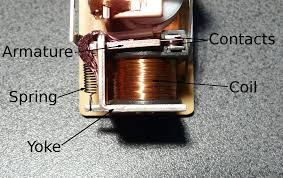
\includegraphics[scale=0.6]{figuras/relay}}
  \subfloat[Diagrama esquemático\label{fig:diagRele}]{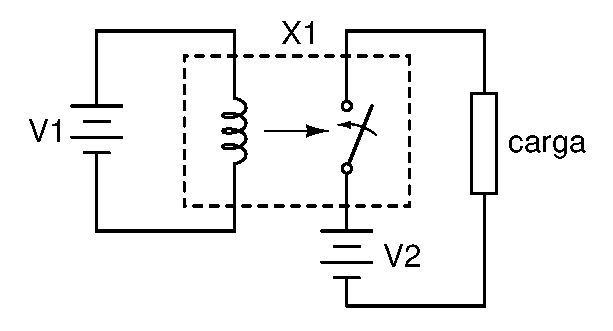
\includegraphics[scale=0.6]{figuras/rele}} %%TODO: refazer
  \caption{Foto de um relê e representação esquemática.}
\end{figure}

Uma grande utilidade dos relês vem do fato que a bobina de acionamento é eletricamente isolada dos cantatos, o que permite usar relês para:
\begin{itemize}
  \item Controle de alta tensão e/ou potência através de baixa tensão e/ou potência -- um sinal de mW pode comandar kW de potência através de um relê.
  \item Isolação e proteção do circuito de controle.
  \item Acionamento trifásico -- um contator é um relê com três conjuntos isolados de contatos acionados pela mesma bobina.
  \item Implementação de lógica de controle -- são os chamados circuitos chaveados.
\end{itemize}
\section{De relês a CLPs}

Um exemplo de aplicação de relê é mostrado na figura \ref{fig:releCircuito1}, onde 2 relês c1 e c2 são usados para o acionamento de um motor trifásico comandado pelas botoeiras b0, b1 e b2.

\begin{figure}[hbt]
  \begin{center}
    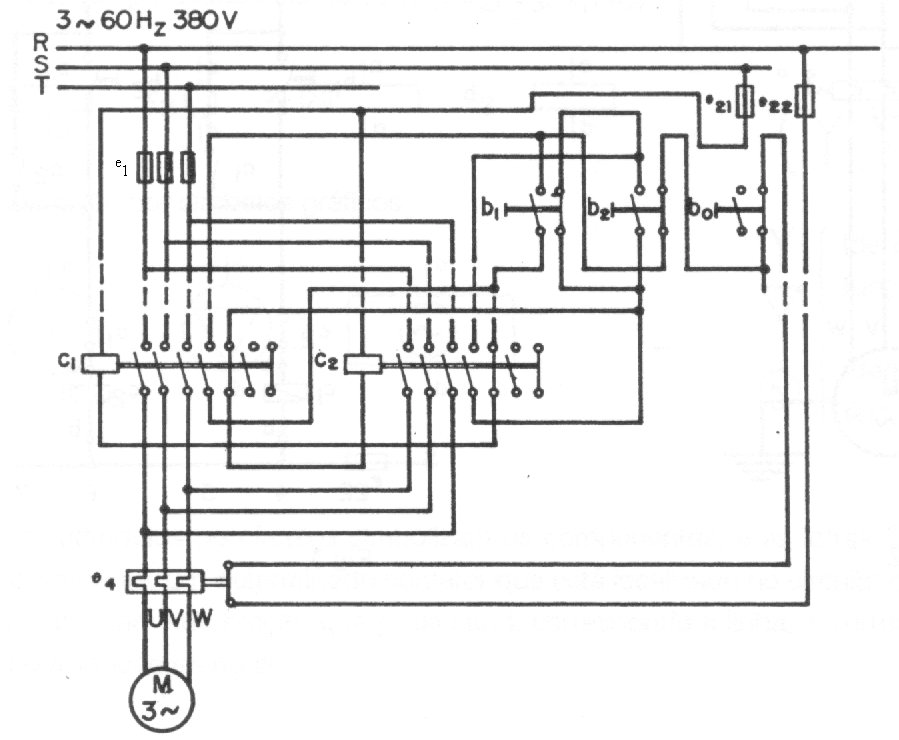
\includegraphics[width=0.8\textwidth]{figuras/releCircuito1} %%TODO: refazer
  \end{center}
  \caption{Circuito de acionamento de um motor trifásico por relê.}
  \label{fig:releCircuito1}
\end{figure}

Em geral é mais fácil analisar um circuito do ponto de vista lógico separando a parte de acionamento da parte de controle, então é comum que o símbolo de um relê seja separado em duas partes: a bobina (o eletroímã) e o contato (a chave), interligados pelo mesmo nome. Isto é exemplificado na figura \ref{fig:releCircuito2}, que redesenha o mesmo circuito da figura \ref{fig:releCircuito1} separando a parte de controle da de acionamento, tornando o circuito bem menos convoluto. A ligação entre os diversos contatos e bobinas dos relês permite a realização de diversas funções interessantes para o controle de circuito. Tais circuitos ficaram conhecidos por \emph{circuitos chaveados}.

\begin{figure}[hbt]
  \begin{center}
    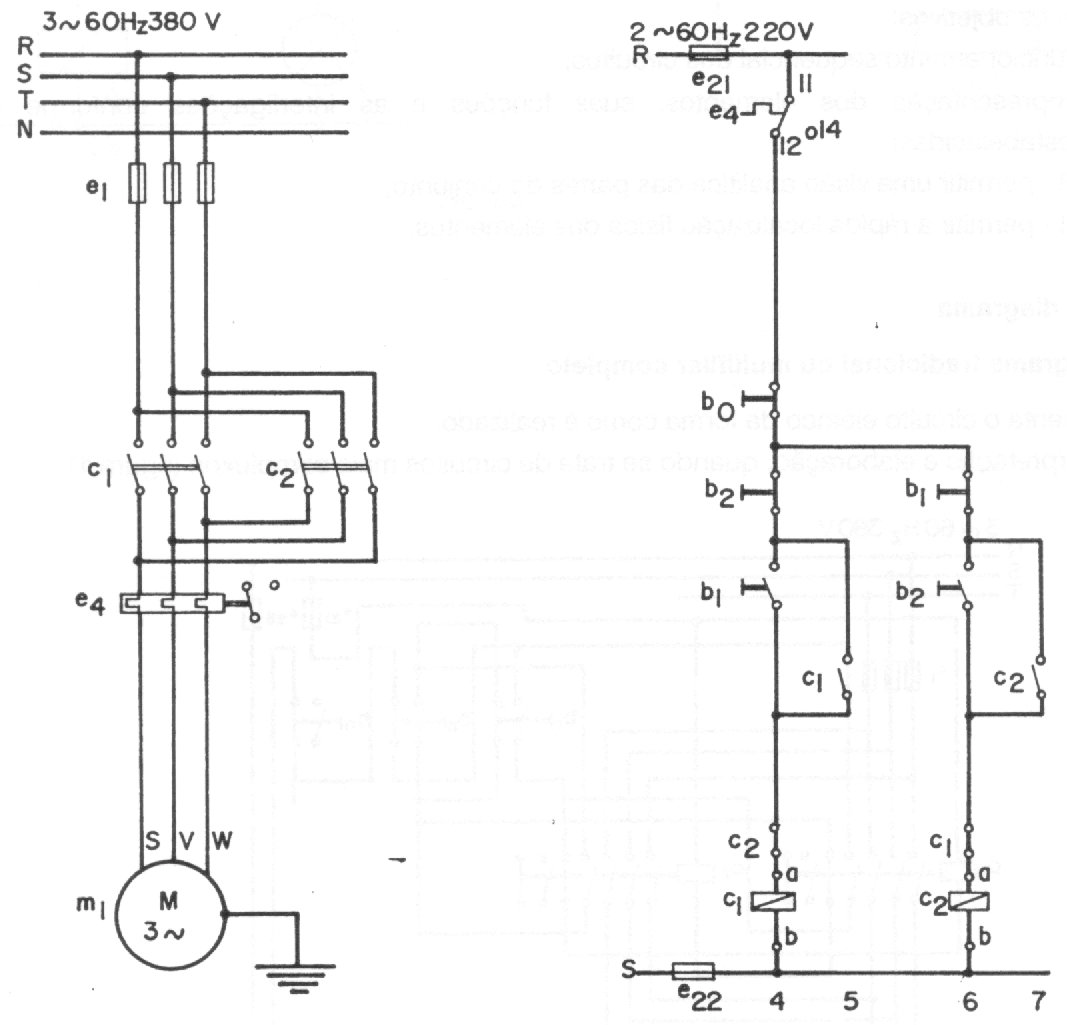
\includegraphics[width=0.8\textwidth]{figuras/releCircuito2} %%TODO: refazer
  \end{center}
  \caption{Mesmo circuito da figura \ref{fig:releCircuito1}, separando a parte de controle da de acionamento.}
  \label{fig:releCircuito2}
\end{figure}

\subsection{Diagrama Ladder}
\label{sec:diagrama-ladder}

Os diagramas ladder são muito utilizados para representar circuitos com relês enfantizando a lógica da ligação. Neste tipo de diagrama as bobinas tem o símbolo 
\includegraphics[height=0.9em]{figuras/bobina_ladder}, os contatos normalmente abertos são simbolizados por 
\includegraphics[height=0.9em]{figuras/na_ladder} e os normalmente fechados por 
\includegraphics[height=0.9em]{figuras/nf_ladder}.

A Figura \ref{fig:ladder1} mostra o mesmo circuito de controle da Figura \ref{fig:releCircuito2}, só que agora descrito em ladder. Com os circuitos conectados desta maneira, o diagrama fica parecendo uma escada; daí o nome\footnote{em inglês \emph{ladder} significa escada.}.


\begin{figure}[!h]
  \centering
  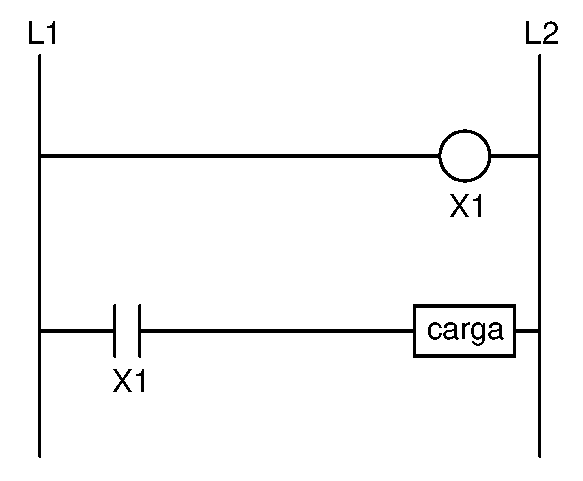
\includegraphics[scale=0.6]{figuras/ladder1} %%TODO: Refazer para ser o mesmo da figura ref:releCircuito2
  \caption{Exemplo de circuito de controle em ladder.}
  \label{fig:ladder1}
\end{figure}

Logo de cara nota-se que não existem neste diagrama as tensões V1 e V2. Isto se dá pois neste diagrama considera-se que as tensões estão entre as duas barras L1 e L2 e abstrai-se a fonte de tensão. Isto lembra, de certo modo, a ligação real, com os elementos conectados entre os cabos de fase e o neutro.


Como exemplo, a figura \ref{fig:ladders} mostra diagramas ladder que acendem uma lâmpada apenas quando 2 relês são acionados, se qualquer um dos relês for acionado ou quando nenhum dos relês é acionado.

\begin{figure}[!h]
  \centering
  \subfloat[Aciona apenas se ambos relês estiverem acionados.]{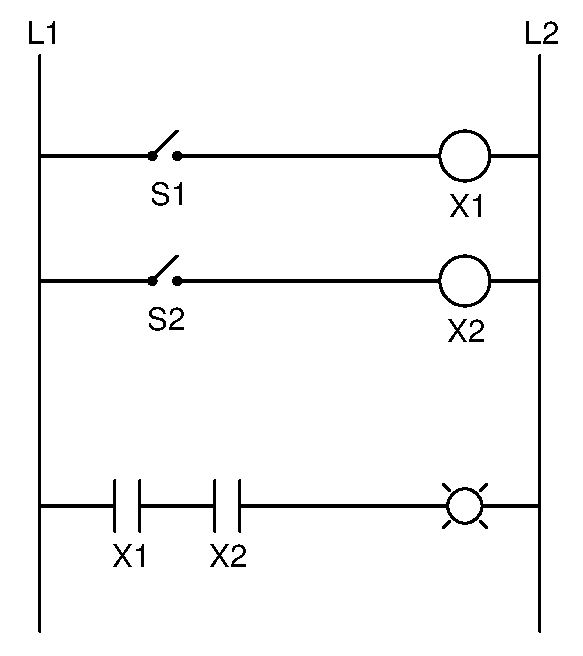
\includegraphics[scale=0.6]{figuras/ladder_e}}
  \subfloat[Aciona se um ou outro relê estiver acionado.]{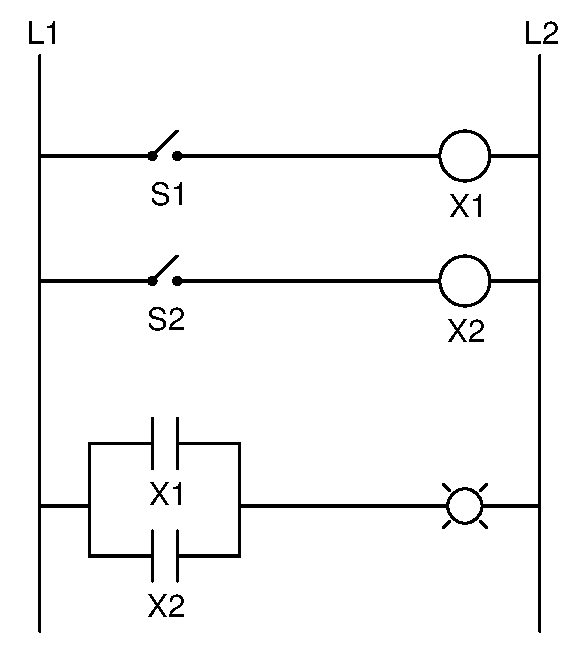
\includegraphics[scale=0.6]{figuras/ladder_ou}}
  \subfloat[Aciona se o relê não estiver acionado.]{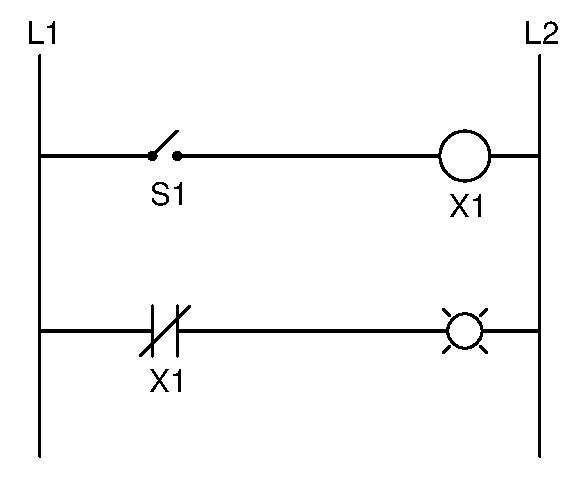
\includegraphics[scale=0.6]{figuras/ladder_nao}}
  \caption{Exemplos de circuitos lógicos chaveados em ladder.}
  \label{fig:ladders}
\end{figure}


O engenheiro Claude Shannon descobriu em 1934 a relação entre os circuitos chaveados e a álgebra de Boole, que é um mapeamento da lógica em uma álgebra. Uma ligação em série realiza um $\mathrm{AND}$ lógico (uma multiplicação booleana), uma ligação paralela realiza um $\mathrm{OR}$ lógico (uma soma na álgebra de Boole) e o uso de um contato normalmente fechado realiza a inversão lógica, ou o $\mathrm{NOT}$ (representado por uma barra sobre a variável). A álgebra de Boole mostra que a combinação destas três operações, e portanto a combinação destes três circuitos, permite realizar qualquer condição lógica para o acionamento do que quer que seja, muito embora a aplicação direta dos postulados e teoremas desta álgebra não seja muito intuitiva.

Porém, apesar da facilidade deste diagrama, a montagem física ainda era bastante complexa, uma vez que o acionamento e os contatos de um relê são obrigatoriamente parte de um único dispositivo físico, e que para lógicas mais complexas essa fiação se tornava bastante complicada. Isto é ainda mais preocupante quando se precisa alterar a lógica de funcionamento, pois se tem que mexer no circuito como um todo.

Além disso, por ser um dispositivo eletromecânico, relês não tem um elevado tempo de vida: pode chavear talvez menos que 10 000 vezes, dependendo da tensão e corrente que suporta.

Em 1947, foi inventado o transistor, que age, como o relê, como uma chave elétrica controlada eletricamente. Principalmente pelo fato de não ter partes móveis, um transistor tem um tempo de vida muito mais longo que um relê, além de ter um chavemaneto mais rápido. Isto permitiu a construção de computadores eletrônicos muito mais rápidos, confiáveis e robustos que os a relê. O problema para o uso na automação é que os transistores não aguentam tensões e correntes tão elevadas quanto os relês.

Em 1968, a GM lançou uma especificação de um elemento de controle que pudesse substituir relês. Esta especificação pedia por:
\begin{itemize}
  \item Facilidade de programação;
  \item Facilidade na manutenção (encaixe de módulos);
  \item Confiabilidade maior;
  \item Mais compacto;
  \item Possibilitar o envio de dados à central de processamento;
  \item Economicamente competitivo;
  \item Entradas em tensão alternada 115 V;
  \item Saídas  em 115 V C.A. com mais que 2 A (operação das válvulas solenóides, comando para partida de motores e outros);
  \item Possibilitar a ampliação com um mínimo de alteração;
  \item Dotado de memória;
\end{itemize}

A partir desta especificação, foi desenvolvido pela Bedford Associates o primeiro PLC, posteriormente vendido pela marca MODICON -- \emph{MOdular DIgital CONtroller}. Ele usa um microcontrolador para realizar a lógica e conta com dispositivos modulares de interface de entrada e saída. A figura \ref{fig:plc_sistema} mostra a arquitetura típica de um CLP.

\begin{figure}[hbt]
  \centering
  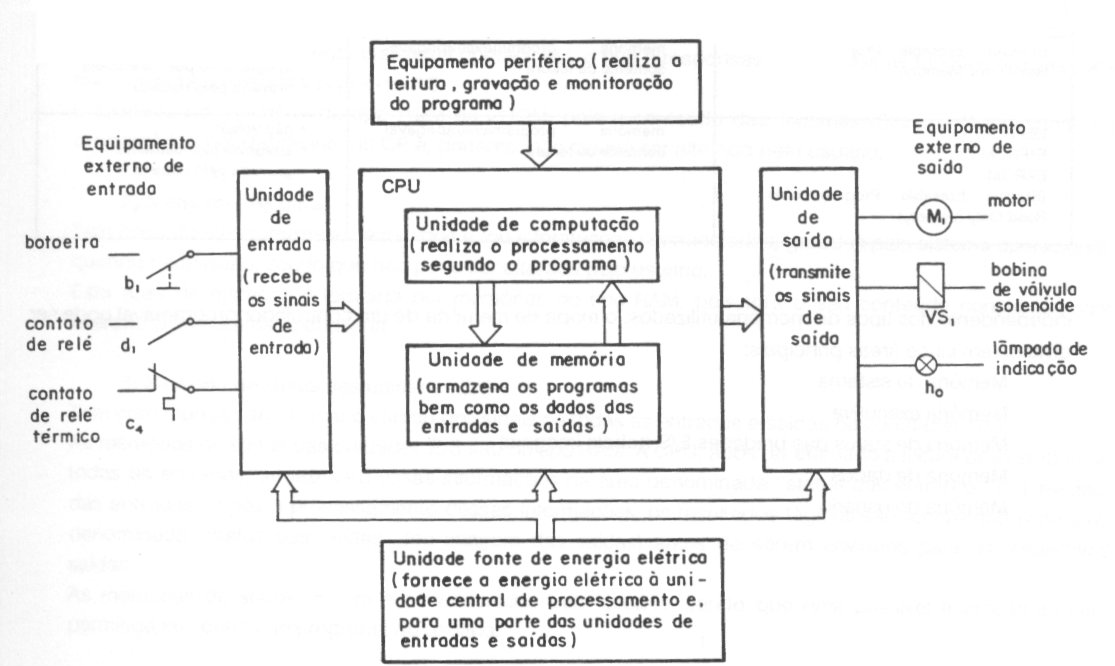
\includegraphics[width=\textwidth]{figuras/plc_sistema}
  \caption{Arquitetura interna de um CLP.}
  \label{fig:plc_sistema}
\end{figure}

As entradas e saídas dos CLPs são isoladas eletricamente, uma vez que o microcontrolador não suporta altas tensões ou correntes. Tipicamente ainda são usados relês para a implementação das saídas digitais, mas cada vez mais se tem soluções totalmente eletrônicas. A Figura \ref{fig:ESclp} mostra circuitos típicos de entrada e saída.
\begin{figure}[h]
  \centering
  \begin{tabular}{cc}
  \subfloat[Entrada de tensão contínua.]{  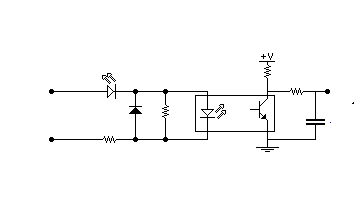
\includegraphics[width=0.45\textwidth]{figuras/entrada_clp_cc}} &
  \subfloat[Entrada de tensão alternada.]{  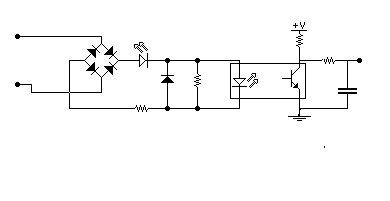
\includegraphics[width=0.45\textwidth]{figuras/entrada_clp_ca}} \\
  \subfloat[Saída a relê.]{  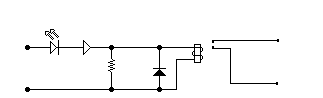
\includegraphics[width=0.45\textwidth]{figuras/saida_clp_rele}} &
  \subfloat[Saída de tensão contínua.]{  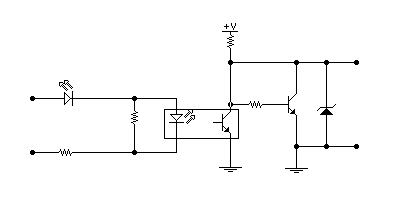
\includegraphics[width=0.45\textwidth]{figuras/saida_clp_cc}}\\
  \end{tabular}
  \caption{Entradas e saídas típicas de CLPs.}
  \label{fig:ESclp}
\end{figure}

%Com este tipo de diagrama, fica fácil analisar a lógica por trás dos circuitos, o que fez com que este diagrama ainda seja usado, só que agora como uma linguagem gráfica de programação de CLPs.

% \section{Mapas de Karnaugh}

% O chamado mapa de Karnaugh foi desenvolvido pelo matemático e físico Maurice Karnaugh em 1953, enquanto trabalhava no grupo de pesquisas da empresa Bell. Este método é uma poderosa ferramenta para circuitos lógicos. %, pois permite simplificar equações booleanas apenas agrupando áreas comuns, o que nosso cérebro consegue fazer bem mais rapidamente do que aplicando postulados e teoremas a equações.

% Como as equações da álgebra de Boole tratam, também, de probabilidade, elas podem ser visualizadas através de um diagrama de Venn. Isto é exemplificado na figura \ref{fig:Venn_mintermos}, que apresenta um diagrama de Venn de 3 variáveis com todas as regiões demarcadas.

% \begin{figure}[!h]
% 	\centering
%   \subfloat[Regiões das variáveis]{\begin{tikzpicture}[scale=1,every node/.style={fill=white,rounded corners}]
%    \draw(0,0)rectangle(4,4);%\draw[step=5mm, red] (0,0) grid (4,4);
%    \draw[pattern=horizontal lines](1.5,1.7)circle(1.2cm);\draw(1,1.2)node{$a$};
%    \draw[pattern=vertical lines](2.5,1.7)circle(1.2cm);\draw(3,1.2)node{$b$};
%    \draw[pattern=north east lines](2,2.5)circle(1.2cm);\draw(2,3.2)node{$c$};
%    \end{tikzpicture}}
% \subfloat[Sub-regiões dos ANDs.]{\begin{tikzpicture}[scale=1,every node/.style={fill=white,rounded corners}]
%    \draw(0,0)rectangle(4,4);%\draw[step=5mm, red] (0,0) grid (4,4);
%    \draw[pattern=horizontal lines](1.5,1.7)circle(1.2cm);
% \draw(1,1.2)node{\scriptsize{$a\comp{b}\comp{c}$}};
%    \draw[pattern=vertical lines](2.5,1.7)circle(1.2cm);
% \draw(3,1.2)node{\scriptsize{$\comp{a}b\comp{c}$}};
%    \draw[pattern=north east lines](2,2.5)circle(1.2cm);
% \draw(2,3.2)node{\scriptsize{$\comp{a}\comp{b}c$}};

%    \draw(2,1)node{\scriptsize{${a}{b}\comp{c}$}};
%    \draw(1.2,2.5)node{\scriptsize{${a}\comp{b}{c}$}};
%    \draw(2.8,2.5)node{\scriptsize{$\comp{a}{b}{c}$}};
%    \draw(2,2)node{\scriptsize{${a}{b}{c}$}};
%    \draw(2,0.25)node{\scriptsize{$\comp{a}\comp{b}\comp{c}$}};
%    \end{tikzpicture}}
% 	\caption{Diagrama Venn com 3 variáveis.}
% 	\label{fig:Venn_mintermos}
% \end{figure}

% Utilizando os diagramas, é fácil obter a equação simplificada da função. Por exemplo, considere-se a função $f_1=a\comp{b}\comp{c}+a\comp{b}c+\comp{a}\comp{b}c$. Desenhando esta função num diagrama de Venn (figura \ref{fig:Venn_f1}), fica óbvio que podemos simplificá-la para $f_1=(a+c)\comp{b}$.

% \begin{figure}[!h]
% 	\centering
% 	\begin{tikzpicture}[scale=1.4,every node/.style={rounded corners}]
%    \coordinate (a) at ($ (2,2)+(-150:0.6cm)$);
%    \coordinate (b) at ($(2,2)+(-30:0.6cm)$);
%    \coordinate (c) at (2,2.6);
%    \draw(0,0)rectangle(4,4);%\draw[step=1mm, red] (0,0) grid (4,4);
%    \node(a1) at (a)[draw,circle,minimum size=2.4*1.4cm]{};%\draw(1,1.2)node{$a$};
%    \node(b1) at (b)[draw,circle,minimum size=2.4*1.4cm]{};
%    \node(c1) at (c)[draw,circle,minimum size=2.4*1.4cm]{};

%    \fill[pattern=north east lines](intersection 1 of a1 and b1)arc(295:125:1.2cm)arc(176:4:1.2cm)arc(55:244:1.2cm);\draw(2,2)+(150:1cm)node[fill=white]{$f_1$};
% \end{tikzpicture}
% 	\caption{Diagrama Venn definindo a região dada por $f_1=a\comp{b}\comp{c}+a\comp{b}c+\comp{a}\comp{b}c=(a+c)\comp{b}$.}
% 	\label{fig:Venn_f1}
% \end{figure}

% O problema aparece quando acrescentamos mais 1 variável. Como fazer um diagrama definindo todas as 16 possibilidades? Uma solução para isto é desenhar as regiões como retângulos e não como círculos, assim como foi feito na figura \ref{fig:Venn4}, lado esquerdo. Uma melhora é ainda aplicada no diagrama do lado direito desta figura, onde a indicação de que regiões correspondem a que variáveis é feita não pelo padrão da área, mas sim indicada no lado externo.

% \begin{figure}[!hbt]
% 	\centering
% %\subfloat{
% \begin{tikzpicture}[scale=1.3,every node/.style={rounded corners,fill=white}]
%   \draw(0,0)rectangle(4,4);%\draw[step=1mm, red] (0,0) grid (4,4);
%   \draw[rounded corners,pattern=north east lines](0.05,0.05)rectangle(3.95,2);
%   \draw[rounded corners,pattern=north west lines](2,0.05)rectangle(3.95,3.95);
%   \draw[rounded corners,pattern=horizontal lines](0.05,1)rectangle(3.95,3);
%   \draw[rounded corners,pattern=vertical lines](1,0.05)rectangle(3,3.95);
% \kmin{\small{$\comp{a}\comp{b}\comp{c}\comp{d}$}}{\small{$\comp{a}\comp{b}\comp{c}{d}$}}{\small{$\comp{a}\comp{b}{c}\comp{d}$}}{\small{$\comp{a}\comp{b}{c}{d}$}}{\small{$\comp{a}{b}\comp{c}\comp{d}$}}{\small{$\comp{a}{b}\comp{c}{d}$}}{\small{$\comp{a}{b}{c}\comp{d}$}}{\small{$\comp{a}{b}{c}{d}$}} %Coloca os valores dos quadros menos significativos
% \kmax{\small{${a}\comp{b}\comp{c}\comp{d}$}}{\small{${a}\comp{b}\comp{c}{d}$}}{\small{${a}\comp{b}{c}\comp{d}$}}{\small{${a}\comp{b}{c}{d}$}}{\small{${a}{b}\comp{c}\comp{d}$}}{\small{${a}{b}\comp{c}{d}$}}{\small{${a}{b}{c}\comp{d}$}}{\small{${a}{b}{c}{d}$}} %Coloca os valores dos quadros mais significativos
% %\end{tikzpicture}}
% %\subfloat{\begin{tikzpicture}[scale=1.2,every node/.style={rounded corners,fill=white}]
% \begin{scope}[xshift=5cm]
%   \draw(0,0)rectangle(4,4);%\draw[step=1mm, red] (0,0) grid (4,4);
%   \draw[rounded corners,](0.05,0.05)rectangle(3.95,2);
%   \draw(-0.1,0)--(-0.1,1)node[left]{$a$}--(-0.1,2);
%  \draw(4.1,1)--(4.1,2)node[right]{$b$}--(4.1,3);
%  \draw(2,-0.1)--(3,-0.1)node[below]{$c$}--(4,-0.1);
%  \draw(1,4.1)--(2,4.1)node[above]{$d$}--(3,4.1);
%   \draw[rounded corners,](2,0.05)rectangle(3.95,3.95);
%   \draw[rounded corners,](0.05,1)rectangle(3.95,3);
%   \draw[rounded corners,](1,0.05)rectangle(3,3.95);
% \kmin{\small{$\comp{a}\comp{b}\comp{c}\comp{d}$}}{\small{$\comp{a}\comp{b}\comp{c}{d}$}}{\small{$\comp{a}\comp{b}{c}\comp{d}$}}{\small{$\comp{a}\comp{b}{c}{d}$}}{\small{$\comp{a}{b}\comp{c}\comp{d}$}}{\small{$\comp{a}{b}\comp{c}{d}$}}{\small{$\comp{a}{b}{c}\comp{d}$}}{\small{$\comp{a}{b}{c}{d}$}} %Coloca os valores dos quadros menos significativos
% \kmax{\small{${a}\comp{b}\comp{c}\comp{d}$}}{\small{${a}\comp{b}\comp{c}{d}$}}{\small{${a}\comp{b}{c}\comp{d}$}}{\small{${a}\comp{b}{c}{d}$}}{\small{${a}{b}\comp{c}\comp{d}$}}{\small{${a}{b}\comp{c}{d}$}}{\small{${a}{b}{c}\comp{d}$}}{\small{${a}{b}{c}{d}$}} %Coloca os valores dos quadros mais significativos
%  \end{scope}
% \end{tikzpicture}
% \caption{Diagrama Venn de 4 variáveis desenhado com regiões quadradas.}
% 	\label{fig:Venn4}
% \end{figure}

% O mapa de Karnaugh já é este diagrama de Venn modificado, onde o resultado da função booleana mapeada é marcado em cada região (casa). Cada casa em um mapa de Karnaugh corresponde a uma linha na tabela verdade, que é um AND de todas as variáveis envolvidas -- vamos chamar isto de mintermo. A figura \ref{fig:karnaugh_mintermos} mostra os mintermos correspondentes a cada uma das regiões.

% \begin{figure}[hbt]
% 	\centering
%   \begin{tikzpicture}[scale=1.2]
%    \karnaugh{$a$}{$b$}{$c$}{$d$} %Faz um mapa de Karnaugh de 0 a 4
%    \kmin{$\comp{a}\comp{b}\comp{c}\comp{d}$}{$\comp{a}\comp{b}\comp{c}{d}$}{$\comp{a}\comp{b}{c}\comp{d}$}{$\comp{a}\comp{b}{c}{d}$}{$\comp{a}{b}\comp{c}\comp{d}$}{$\comp{a}{b}\comp{c}{d}$}{$\comp{a}{b}{c}\comp{d}$}{$\comp{a}{b}{c}{d}$} %Coloca os valores dos quadros menos significativos
%    \kmax{${a}\comp{b}\comp{c}\comp{d}$}{${a}\comp{b}\comp{c}{d}$}{${a}\comp{b}{c}\comp{d}$}{${a}\comp{b}{c}{d}$}{${a}{b}\comp{c}\comp{d}$}{${a}{b}\comp{c}{d}$}{${a}{b}{c}\comp{d}$}{${a}{b}{c}{d}$} %Coloca os valores dos quadros mais significativos
% 	 \end{tikzpicture}
% 	\caption{Mapa de Karnaugh com os mintermos correspondentes a cada casa.}
% 	\label{fig:karnaugh_mintermos}
% \end{figure}

% Note na figura \ref{fig:karnaugh_mintermos} que os vizinhos de cada casa em um mapa de Karnaugh são tais que apenas muda uma variável de cada vez. Por exemplo, da casa 5 para a 1 (acima) só muda o $b$, da 5 para a 7 (direita) só muda o $c$, da 5 para a 4 (esquerda) só muda o $d$ e da 5 para a 13 (abaixo) só muda o $a$.

% Isto que foi mostrado para a casa 5 é válido para todas casas, inclusive para as bordas e quinas, pois podemos considerar que o mapa dá a volta em si mesmo. Deste modo considera-se a casa 6 como vizinha da 4 e só muda a variável $c$, a casa 10 vizinha da 2 e só muda a variável $a$ e assim por diante.

% Desta característica do mapa de Karnaugh vem sua principal utilidade. Por exemplo, considere a função $f_2=\Sigma_m(3,7,12,13)$ -- o somatório dos mintermos das casas 3, 7, 12 e 13 -- e seu respectivo mapa de karnaugh na figura \ref{fig:k_f2}.

% \begin{figure}[hbt]
% 	\centering
%   \begin{tikzpicture}[scale=0.8]
%     \node() at(0,4)[above left]{$f_2=\Sigma_m(3,7,12,13)$};
%    \karnaugh{$a$}{$b$}{$c$}{$d$} %Faz um mapa de Karnaugh de 0 a 4
%    \kmin{0}{0}{0}{1}{0}{0}{0}{1} %Coloca os valores dos quadros menos significativos
%    \kmax{0}{0}{0}{0}{1}{1}{0}{0} %Coloca os valores dos quadros mais significativos
%    \grupo{0}{1}{2}{2}\node(p1)at (0.1,1.5){};
%    \node(e1) at (-2,2){$ab\comp{c}$} edge[->,thick](p1);
% 	 \grupo{2}{2}{3}{4}\node(p2)at (2.9,3){};
% 	 \node(e2) at (6,3.5){$\comp{a}cd$} edge[->, thick](p2);
% 	 \end{tikzpicture}
% 	\caption{Função $f_2$ e simplificação por agrupamento de casas vizinhas.}
% 	\label{fig:k_f2}
% \end{figure}

% Analisando a função $f_2$ por álgebra de Boole, vemos que podemos simplificá-la através da aplicação do teorema que diz que $a\comp{b}+ab=a$ e, observando no mapa de Karnaugh, os termos que são unidos e simplificados são justamente os vizinhos.
% \begin{equation*}
% \begin{matrix}
% f_2=&\!\!\!\underbrace{\comp{a}\comp{b}cd+\comp{a}bcd}&\!\!\!\!+&\!\!\!\!\underbrace{ab\comp{c}\comp{d}+ab\comp{c}d}\\
% f_2=&\!\!\comp{a}cd&\!\!\!\!+&ab\comp{c}
% \end{matrix}
% \end{equation*}

% Ou seja, o agrupamento de 2 casas vizinhas corresponde à simplificação de uma variável. Basta ver no próprio mapa quais são as variáveis que não mudam dentro do agrupamento.

% Para simplificar 2 ou mais variáveis basta aplicar o teorema repetidas vezes. Simplifiquemos a função $f_3$ (vide figura \ref{fig:k_g_simples}), por exemplo. Basta agruparmos a função de duas em duas casas e 2 grupos vizinhos de duas casas viram um único grupo de 4 casas, retirando mais uma variável da função.

% \begin{figure}[hbt]
% \begin{align*}
% f_3&=\underbrace{a\comp{b}\comp{c}\comp{d}+a\comp{b}\comp{c}{d}}+\underbrace{a{b}\comp{c}\comp{d}+a{b}\comp{c}{d}}\\
%  &=\underbrace{a\comp{b}\comp{c}+a{b}\comp{c}}\\
%  f_3&=a\comp{c}
% \end{align*}
% 	\centering

% \begin{center}
% %	\begin{tabular}[c]{cc}
%   \begin{tikzpicture}[scale=0.8]
%     \node() at (0,4)[above left]{$f_3$};
%    \karnaugh{$a$}{$b$}{$c$}{$d$} %Faz um mapa de Karnaugh de 0 a 4
%    \kmin{0}{0}{0}{0}{0}{0}{0}{0} %Coloca os valores dos quadros menos significativos
%    \kmax{1}{1}{0}{0}{1}{1}{0}{0} %Coloca os valores dos quadros mais significativos
%    \grupo{0}{0}{2}{1}\node(p1)at (0.1,1.5){};
%    \grupo{0}{1}{2}{2}\node(p1)at (0.1,1.5){};
% %   \end{tikzpicture} %&
% %		  \begin{tikzpicture}[scale=0.8]
%    \node(seta) at (6,2){\Huge $\Rightarrow$};
% 		\begin{scope}[xshift=8cm]
%     \node() at (0,4)[above left]{$f_3$};
%    \karnaugh{$a$}{$b$}{$c$}{$d$} %Faz um mapa de Karnaugh de 0 a 4
%    \kmin{0}{0}{0}{0}{0}{0}{0}{0} %Coloca os valores dos quadros menos significativos
%    \kmax{1}{1}{0}{0}{1}{1}{0}{0} %Coloca os valores dos quadros mais significativos
%    \grupo{0}{0}{2}{2}\node(p1)at (0.1,1.5){};
%    \end{scope}
%    \end{tikzpicture}
% %	\end{tabular}
% \end{center}
% 	\caption{Agrupamento das casas da função $f_3$.}
% 	\label{fig:k_g_simples}
% \end{figure}

% Este mesmo procedimento pode ser mostrado para agrupamentos de 8 casas (simplificando então 3 variáveis) ou 16 casas (simplificando 4 variáveis.
% A figura \ref{fig:k_exemplos}\footnote{Exemplos retirados do artigo original de Karnaugh: ``\emph{The map method for synthesis of combinational logic circuits}'', de 1953.} mostra algumas possibilidades de agrupamentos de 2, 4 e 8 casas, junto com o produto respectivo. Num mapa de Karnaugh de 4 variáveis um agrupamento de 16 casas seria todo o mapa e corresponderia a função 1.

% \begin{figure}[hbtp]\begin{center}%
% \subfloat[agrupamentos de 2 casas]{
%  \begin{tikzpicture}[scale=0.4]
%    \draw(-0.1,4.1)node[above left]{$b\comp{c}d$};
%    \karnaugh[0]{$a$}{$b$}{$c$}{$d$} %Faz um mapa de Karnaugh de 0 a 4
%    \kmin{0}{0}{0}{0}{0}{1}{0}{0} %Coloca os valores dos quadros menos significativos
%    \kmax{0}{0}{0}{0}{0}{1}{0}{0} %Coloca os valores dos quadros mais significativos
%    \grupo[indefinido, rounded corners=1.5mm]{1}{1}{2}{3};
% %   \quinas[indefinido, rounded corners=1.5mm]\node(p2)at (0.1,1.5){};
% %   \end{tikzpicture}

% \begin{scope}[xshift=6cm]
%    \draw(-0.1,4.1)node[above left]{$\comp{a}\comp{b}d$};
%    \karnaugh[0]{$a$}{$b$}{$c$}{$d$} %Faz um mapa de Karnaugh de 0 a 4
%    \kmin{0}{1}{0}{1}{0}{0}{0}{0} %Coloca os valores dos quadros menos significativos
%    \kmax{0}{0}{0}{0}{0}{0}{0}{0} %Coloca os valores dos quadros mais significativos
%    \grupo[indefinido, rounded corners=1.5mm]{1}{3}{3}{4}\node(p1)at (0.1,1.5){};
% %   \grupo[indefinido, rounded corners=1.5mm]{1}{0}{2}{4}\node(p2)at (0.1,1.5){};
%    \end{scope}
% \begin{scope}[xshift=12cm]
%    \draw(-0.1,4.1)node[above left]{$\comp{a}\comp{b}\comp{d}$};
%    \karnaugh[0]{$a$}{$b$}{$c$}{$d$} %Faz um mapa de Karnaugh de 0 a 4
%    \kmin{1}{0}{1}{0}{0}{0}{0}{0} %Coloca os valores dos quadros menos significativos
%    \kmax{0}{0}{0}{0}{0}{0}{0}{0} %Coloca os valores dos quadros mais significativos
%    \lados[indefinido, rounded corners=1.5mm]{3}{4};

%    \end{scope}
% \begin{scope}[xshift=18cm]
%    \draw(-0.1,4.1)node[above left]{$\comp{b}\comp{c}\comp{d}$};
%    \karnaugh[0]{$a$}{$b$}{$c$}{$d$} %Faz um mapa de Karnaugh de 0 a 4
%    \kmin{1}{0}{0}{0}{0}{0}{0}{0} %Coloca os valores dos quadros menos significativos
%    \kmax{1}{0}{0}{0}{0}{0}{0}{0} %Coloca os valores dos quadros mais significativos
%    \topos[indefinido, rounded corners=1.5mm]{0}{1}\node(p1)at (0.1,1.5){};
% %   \grupo[indefinido, rounded corners=1.5mm]{1}{0}{2}{4}\node(p2)at (0.1,1.5){};
%    \end{scope}
% \end{tikzpicture}}
% \subfloat[Agrupamentos de 4 casas]{
%  \begin{tikzpicture}[scale=0.4]
%  \begin{scope}
%    \draw(-0.1,4.1)node[above left]{$\comp{c}d$};
%    \karnaugh[0]{$a$}{$b$}{$c$}{$d$} %Faz um mapa de Karnaugh de 0 a 4
%    \kmin{0}{1}{0}{0}{0}{1}{0}{0} %Coloca os valores dos quadros menos significativos
%    \kmax{0}{1}{0}{0}{0}{1}{0}{0} %Coloca os valores dos quadros mais significativos
%    \grupo[indefinido, rounded corners=1.5mm]{1}{0}{2}{4};

%  \begin{scope}[xshift=6cm]
%    \draw(-0.1,4.1)node[above left]{$a\comp{b}$};
%    \karnaugh[0]{$a$}{$b$}{$c$}{$d$} %Faz um mapa de Karnaugh de 0 a 4
%    \kmin{0}{0}{0}{0}{0}{0}{0}{0} %Coloca os valores dos quadros menos significativos
%    \kmax{1}{1}{1}{1}{0}{0}{0}{0} %Coloca os valores dos quadros mais significativos
%    \grupo[indefinido, rounded corners=1.5mm]{0}{0}{4}{1};
%      \end{scope}
%  \begin{scope}[xshift=12cm]
%    \draw(-0.1,4.1)node[above left]{$\comp{a}\,\comp{d}$};
%    \karnaugh[0]{$a$}{$b$}{$c$}{$d$} %Faz um mapa de Karnaugh de 0 a 4
%    \kmin{1}{0}{1}{0}{1}{0}{1}{0} %Coloca os valores dos quadros menos significativos
%    \kmax{0}{0}{0}{0}{0}{0}{0}{0} %Coloca os valores dos quadros mais significativos
%    \lados[indefinido, rounded corners=1.5mm]{2}{4};
%      \end{scope}
%  \begin{scope}[xshift=18cm]
%    \draw(-0.1,4.1)node[above left]{$\comp{b}\,\comp{d}$};
%    \karnaugh[0]{$a$}{$b$}{$c$}{$d$} %Faz um mapa de Karnaugh de 0 a 4
%    \kmin{1}{0}{1}{0}{0}{0}{0}{0} %Coloca os valores dos quadros menos significativos
%    \kmax{1}{0}{1}{0}{0}{0}{0}{0} %Coloca os valores dos quadros mais significativos
%    \quinas[indefinido, rounded corners=1.5mm];
%      \end{scope}
%    \end{scope}
% \end{tikzpicture}}
% \subfloat[Agrupamentos de 8 casas]{
%  \begin{tikzpicture}[scale=0.4]
%  \begin{scope}
%    \draw(-0.1,4.1)node[above left]{$b$};
%    \karnaugh[0]{$a$}{$b$}{$c$}{$d$} %Faz um mapa de Karnaugh de 0 a 4
%    \kmin{0}{0}{0}{0}{1}{1}{1}{1} %Coloca os valores dos quadros menos significativos
%    \kmax{0}{0}{0}{0}{1}{1}{1}{1} %Coloca os valores dos quadros mais significativos
%    \grupo[indefinido, rounded corners=1.5mm]{0}{1}{4}{3};

%  \begin{scope}[xshift=6cm]
%    \draw(-0.1,4.1)node[above left]{$\comp{d}$};
%    \karnaugh[0]{$a$}{$b$}{$c$}{$d$} %Faz um mapa de Karnaugh de 0 a 4
%    \kmin{1}{0}{1}{0}{1}{0}{1}{0} %Coloca os valores dos quadros menos significativos
%    \kmax{1}{0}{1}{0}{1}{0}{1}{0} %Coloca os valores dos quadros mais significativos
%    \lados[indefinido, rounded corners=1.5mm]{0}{4};
%      \end{scope}
%  \begin{scope}[xshift=12cm]
%    \draw(-0.1,4.1)node[above left]{$c$};
%    \karnaugh[0]{$a$}{$b$}{$c$}{$d$} %Faz um mapa de Karnaugh de 0 a 4
%    \kmin{0}{0}{1}{1}{0}{0}{1}{1} %Coloca os valores dos quadros menos significativos
%    \kmax{0}{0}{1}{1}{0}{0}{1}{1} %Coloca os valores dos quadros mais significativos
%    \grupo[indefinido, rounded corners=1.5mm]{2}{0}{4}{4};
%      \end{scope}
%  \begin{scope}[xshift=18cm]
%    \draw(-0.1,4.1)node[above left]{$\comp{b}$};
%    \karnaugh[0]{$a$}{$b$}{$c$}{$d$} %Faz um mapa de Karnaugh de 0 a 4
%    \kmin{1}{1}{1}{1}{0}{0}{0}{0} %Coloca os valores dos quadros menos significativos
%    \kmax{1}{1}{1}{1}{0}{0}{0}{0} %Coloca os valores dos quadros mais significativos
%    \topos[indefinido, rounded corners=1.5mm]{0}{4};
%      \end{scope}
%    \end{scope}
%    \end{tikzpicture}}
% \caption{Exemplos de mapas de karnaugh com os correspondentes produtos algébricos.}\label{fig:k_exemplos}
% \end{center}
% \end{figure}
% \clearpage

% \subsection{Mapas de $n$ variáveis}

% É fácil fazer um mapa de Karnaugh com um número menor de variáveis (i.e.: $n<4$). Para tanto basta simplesmente sair dividindo o mapa. Deve-se apenas lembrar que uma casa deve ter $n$ vizinhas, já que a simplificação de uma variável corresponde a unir uma casa com a vizinha. Isto é mostrado na figura \ref{fig:karnaughzinhos} para mapas de 2, 3 e 4 variáveis.

% \begin{figure}[!h]
% \centering
% \subfloat[Mapa de 2 variáveis]{
%  \begin{tikzpicture}[scale=0.7]
% \draw[step=1cm, black] (0,0) grid (2,2); %defining grids
%   \draw(-0.1,0)--(-0.1,0.5)node[left]{$a$}--(-0.1,1);
%   \draw(1,-0.1)--(1.5,-0.1)node[below]{$b$}--(2,-0.1);

%   \draw(1,1)node[above left]{\scriptsize 0};
%   \draw(2,1)node[above left]{\scriptsize 1};
%   \draw(1,0)node[above left]{\scriptsize 2};
%   \draw(2,0)node[above left]{\scriptsize 3};
%   \draw[<->](1.5,0.6)--(1.5,1.4);
%   \draw[<->](0.6,0.5)--(1.4,0.5);
%  \end{tikzpicture}}
% \subfloat[Mapa de 3 variáveis]{
%  \begin{tikzpicture}[scale=0.7]
%    \karnaughtres{$a$}{$b$}{$c$}
%    \draw[<->](1.5,0.6)--(1.5,1.4);
%    \draw[<->](0.6,0.5)--(1.4,0.5);
%    \draw[<->](1.6,0.5)--(2.4,0.5);
%  \end{tikzpicture}}
% \subfloat[Mapa de 4 variáveis]{
%  \begin{tikzpicture}[scale=0.7]
%    \karnaugh[1]{$a$}{$b$}{$c$}{$d$} %Faz um mapa de Karnaugh de 0 a 4
%    \draw[<->](1.5,2.6)--(1.5,3.4);
%    \draw[<->](1.5,1.6)--(1.5,2.4);
%    \draw[<->](0.6,2.5)--(1.4,2.5);
%    \draw[<->](1.6,2.5)--(2.4,2.5);
%  \end{tikzpicture}}
% \caption{Mapas de Karnaugh de $n= 2, 3, 4$ variáveis, mostrando que cada casa tem $n$ vizinhas.}
% \label{fig:karnaughzinhos}
% \end{figure}

% Mas como aplicar este princípio para funções com mais de 4 variáveis? É impossível fazer um mapa no plano onde cada uma das regiões tem 5 (ou mais) vizinhos. Uma maneira (não muito prática) é trabalhar com um mapa tridimensional como exemplifica a figura \ref{fig:karnaugh6_3d} que mostra um mapa de Karnaugh de 6 variáveis, note que cada casa tem 6 vizinhos: 4 no plano (como no mapa de 4 variáveis) e 2 verticais.

% \begin{figure}
% \centering

%  \begin{tikzpicture}
%   \begin{scope}[yscale=0.4,xshift=0cm,xslant=0.5]
%    \karnaugh[3]{$c$}{$d$}{$e$}{$f$}
%   \end{scope}
%   \begin{scope}[yshift=2.25cm,yscale=0.4,xshift=0cm,xslant=0.5]
%    \karnaugh[4]{$c$}{$d$}{$e$}{$f$}
%   \end{scope}
%   \begin{scope}[yshift=4.5cm,yscale=0.4,xshift=0cm,xslant=0.5]
%    \karnaugh[2]{$c$}{$d$}{$e$}{$f$}
%   \end{scope}
%   \begin{scope}[yshift=6.75cm,yscale=0.4,xshift=0cm,xslant=0.5]
%    \karnaugh[1]{$c$}{$d$}{$e$}{$f$}
%   \end{scope}
% \draw(-0.25,-0.25)--(-0.25,2)node[left]{$a$}--(-0.25,4.25);
% \draw(6.25,2)--(6.25,4.25)node[right]{$b$}--(6.25,6.5);
% %\draw[color=white](-1,0)--(-1.5,1);

%  \end{tikzpicture}
% \caption{Mapa de Karnaugh tridimensional de 6 variáveis.}\label{fig:karnaugh6_3d}
% \end{figure}


% Na prática, um mapa de 5 variáveis é desenhado como 2 de 4 variáveis, sendo um com uma variável (em geral a mais significativa) sendo 0 e o outro com a mesma variável sendo 1. Usa-se este mesmo princípio para mapas de 6 ou mais variáveis, como pode ser visto na figura \ref{fig:karnaughzaos}.

% \begin{figure}
% \centering
% \subfloat[5 variáveis]{
%  \begin{tikzpicture}[scale=0.45]
%   \begin{scope}[xshift=0cm]
%    \karnaugh[1]{$b$}{$c$}{$d$}{$e$}
%   \end{scope}
%   \begin{scope}[yshift=0cm,xshift=6cm]
%    \karnaugh[2]{$b$}{$c$}{$d$}{$e$}
%   \end{scope}
% \draw(5.5,5.5)--(8,5.5)node[above]{$a$}--(10.5,5.5);
% \end{tikzpicture}
% }
% \subfloat[6 variáveis]{
%  \begin{tikzpicture}[scale=0.45]
%   \begin{scope}[xshift=0cm]
%    \karnaugh[3]{$c$}{$d$}{$e$}{$f$}
%   \end{scope}
%   \begin{scope}[yshift=0cm,xshift=6cm]
%    \karnaugh[4]{$c$}{$d$}{$e$}{$f$}
%   \end{scope}
%   \begin{scope}[yshift=6cm,xshift=6cm]
%    \karnaugh[2]{$c$}{$d$}{$e$}{$f$}
%   \end{scope}
%   \begin{scope}[yshift=6cm,xshift=0cm]
%    \karnaugh[1]{$c$}{$d$}{$e$}{$f$}
%   \end{scope}
% \draw(-1.5,-0.5)--(-1.5,2)node[left]{$a$}--(-1.5,4.5);
% \draw(5.5,11.5)--(8,11.5)node[above]{$b$}--(10.5,11.5);


%  \end{tikzpicture}}
% \caption{Mapas de Karnaugh de 5 e 6 variáveis.}\label{fig:karnaughzaos}
% \end{figure}
% \clearpage

% \section{Equações e circuitos não-completamente especificados.}
% \label{sec:nao-completamente}

% É bastante comum a situação de que determinadas entradas de um circuito lógico nunca ocorram. Como exemplo imagine-se uma esteira carregando uma caixa de um lado para o outro, com sensores de fim de curso em ambas extremidades: $s_e$ do lado esquerdo e $s_d$ do lado direito. No funcionamento normal do sistema estes dois sinais nunca serão acionados ao mesmo tempo; nesta situação não importa qual é o resultado do circuito para $s_e=s_d=1$, já que esta situação nunca vai existir. Diz-se então que este circuito é não-completamente especificado.

% A tabela \ref{tab:verdade_nce} mostra o exemplo de um sinal imaginário $z$ determinado em função de $a$, $s_e$ e $s_d$. Neste exemplo, sempre que $s_e=s_d=1$ a saída $z$ é não-especificada, ou seja, $z$ \emph{não-importa} nestas situações. Neste texto utilizaremos a notação `$\times$' para identificar as situações que um sinal não importa. Outras notações comumente usadas são `$\ast$', `-' ou `$d$'.

% \begin{table}[!h]
%   \centering
%   \caption{Exemplo de uma função não completamente especificada.}
%   \label{tab:verdade_nce}
%     \begin{tabular}{|c|c|c||c|}
% \hline
% $a$ & $s_e$ & $s_d$ & $z$ \\
% \hline\hline
% 0 & 0 & 0 & 0 \\

% 0 & 0 & 1 & 0 \\

% 0 & 1 & 0 & 1 \\

% 0 & 1 & 1 & $\times$ \\
% \hline
% 1 & 0 & 0 & 1 \\

% 1 & 0 & 1 & 0 \\

% 1 & 1 & 0 & 1 \\

% 1 & 1 & 1 & $\times$ \\
% \hline
% \end{tabular}
% \end{table}

% Pode-se descrever uma função lógica não-completamente especificada na forma soma de mintermos utilizando a notação $d(\cdots)$, que vem do inglês \emph{don't care}. Desta forma o sinal z pode ser descrito por:
% \begin{equation}
%   \label{eq:z}
%   z = \Sigma_m(2,4,6)+d(3,7)
% \end{equation}

% Um \dontcare~na saída pode ser implementado como um 1 ou um 0, e não se sabe a princípio qual destes dois valores gerará uma solução mais minimizada, logo para obter o menor circuito possível o engenheiro deveria, a princípio, obter as equações considerando que cada \dontcare~pode ser 1 ou 0 e checar qual é o menor circuito final. Obviamente para problemas com muitos \dontcare's isto se torna impraticável, pois seria necessário minimizar $2^k$ funções, onde $k$ é o número de \dontcare's presentes.

% O mapa de Karnaugh facilita bastante a implementação de circuitos não-completamente especificados, pois podemos considerar se determinado \dontcare~é 1 ou 0 visualmente, na hora da implementação.


% \begin{figure}[!h]
%   \centering
%   \begin{tikzpicture}
%     \node() at (0,2)[above left]{$z$};
%     \karnaughtres{$a$}{$s_e$}{$s_d$}
%     \kmax{1}{0}{1}{$\times$}{0}{0}{1}{$\times$}

% %    \grupo[zeros]{1}{0}{3}{2}
% %    \grupo[zeros]{0}{1}{2}{2}

%     \grupo{2}{0}{4}{2}
%     \lados{0}{1}

%   \end{tikzpicture}
%   \caption{Mapa de Karnaugh da função $z$.}
%   \label{fig:kmap_z}
% \end{figure}
